This part of the book offers our most important insights into peer
learning. A number of earlier theories and experiments have focused on
various aspects of collaborative, connective, and shared, non-didactic
learning systems. There's a rumbling among several well-known thinkers
that when combined with new technologies, peer learning strategies could
have a big impact on the way educational institutions work in the
future. Our aim here is just to make the basic ideas concretely
understandable and immediately applicable. The best course is to try it
out and see how it works for you.

\begin{center}
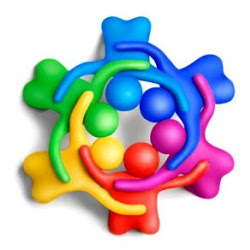
\includegraphics[width=.4\textwidth]{./pictures/peeragogy-in-action.jpg}
\end{center}

Peeragogy is about peers learning together and helping each other learn.
The idea is that each person contributes to the group in their own way.
The contribution of each peeragogue depends on a healthy sense of
self-awareness. You ask yourself, ``What do I have to offer?'' and
``What do I get out of it?'' We think you'll come up with some exciting
answers to those questions!

Our first strategy for peer learning invites you to engage in a
self-assessment of your motivations. Here you take into account things
like the learning context, timing and sequence of learning activities,
social reinforcements, and visible reward. Our view is that learning is
most effective when it contains some form of enjoyment or satisfaction,
or when it leads to a concrete accomplishment.

Indeed, this is the kind of learning that you choose to do, whether
you're being ``trained'' or not. You're in charge! Furthermore, this
kind of learning is usually fun. Indeed, as we'll describe below, there
are deep links between play and learning. We believe we can improve the
co-learning experience by adopting a playful mindset. Certainly some of
our best learning moments in the~Peeragogy project have been peppered
with humor and banter.

Apart from self-assessment and playfulness, here are two key factors to
keep in mind:

\textbf{``Personal'' supports ``peer'':} We can consciously cultivate
living, growing, responsive webs of information, support, and
inspiration that help us be more effective learners. This is a
``personal learning network''.~We'll offer tips on how to build these
networks -- and we'll also explain how strong personal learning networks
can evolve into even stronger \emph{peer} learning networks.

\textbf{``Peer'' supports ``personal'':} As we work together to develop
shared plans or ``roadmaps'' for our collective efforts in group
projects, we usually can find places where we have something to offer,
and places where we have something to learn. Furthermore, if we are
willing to ask for some help and offer our help to others, then we can
really learn a lot! This is why building effective \emph{inter}personal
learning strategies should be part of your personal learning plan.

In the following sections, you can read some more about these
strategies, or you can skip ahead to
\href{http://peeragogy.org/peeragogy-in-action/}{Part III} to start
looking at techniques you can use to build your own peer learning group.

\subsection{Peer learning through the ages}

The new term, ``peeragogy,'' that we use in this book is a riff on the
word pedagogy --- the art, science, or profession of teaching. Pedagogy
has a somewhat problematic story of origin: it comes from the ancient
Greek tradition of having a child (paidos) be supervised (agogos) by a
slave. Greek philosophers disagreed with each other as to the best way
for individuals to gain knowledge (and even more so, wisdom). Socrates,
who insisted that he was not wise, also insisted that his interlocutors
join him in investigating truth claims, as peers. The most famous of
these interlocutors, Plato, on a more pedagogical bent, spoke of an
enlightened few, whose responsibility it was to show others the light of
knowledge (illustrated by his famous allegory of ``The Cave'').

In more recent centuries, various education theorists and reformers have
challenged the effectiveness of what had become the traditional
teacher-led model. Most famous of the early education reformers in the
United States was John Dewey, who advocated new experiential learning
techniques. In his 1916 book, \emph{Democracy and Education}{[}1{]},
Dewey wrote, ``Education is not an affair of `telling' and being told,
but an active and constructive process.'' Soviet psychologist Lev
Vygotsky, who developed the concept of the Zone of Proximal Development,
was another proponent of ``constructivist'' learning. His book,
\emph{Thought and Language}, also gives evidence to support
collaborative, socially meaningful, problem-solving activities over solo
exercises {[}2{]}.

Within the last few decades, things have begun to change very rapidly.
In \emph{Connectivism: A Learning Theory for the Digital Age}, George
Siemens argues that technology has changed the way we learn, explaining
how it tends to complicate or expose the limitations of the learning
theories of the past {[}3{]}. The crucial point of connectivism is that
the connections that make it possible for us to learn in the future are
more relevant than the sets of knowledge we know individually, in the
present. Furthermore, technology can to some degree and in certain
contexts, replace know-how with know-where-to-look.

If you want more details on the history, theories, and recent
experiments related to peer learning, we have a more extensive
\href{http://peeragogy.org/resources/literature-review-peeragogy/}{literature
review} available. We've also adapted it into
\href{http://en.wikipedia.org/wiki/Peer\_learning}{Wikipedia page},
which you can edit as well as read.

\begin{figure}
\href{http://commons.wikimedia.org/wiki/File:Platon\_Cave\_Sanraedam\_1604.jpg}{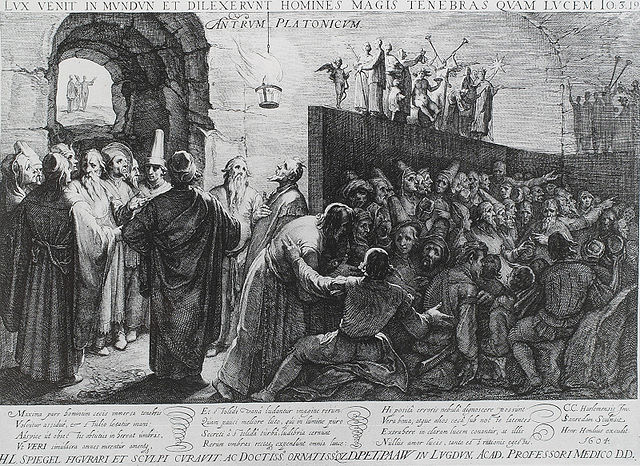
\includegraphics[width=\textwidth]{./pictures/plato_cave.jpg}}
 \caption{\href{http://commons.wikimedia.org/w/index.php?title=File:Platon\_Cave\_Sanraedam\_1604.jpg\&oldid=68567627}{Platon Cave Sanraedam (1604)}. By Jan Saenredam {[}Public domain{]}, via
 Wikimedia Commons}
\end{figure}

\subsection{What makes learning fun? (Or boring, as the case may be!)}

Individuals learn by doing in a continuous process. This is most
effective when it contains some form of enjoyment, satisfaction, or
accomplishment. So for each peer-learning participant, there's a simple
question: ''What makes learning fun for \emph{me}?''

\subsubsection{Two learning stories}

\begin{enumerate}
\item
  A study group for a tough class in neuropsychology convenes at at the
  library late one night, resolving to do well on the next day's exam.
  The students manage to deflect their purpose for a while by gossiping
  about college hook-ups and parties, studying for other classes, and
  sharing photos. Then, first one member, then another, takes the
  initiative and as a group, the students eventually pull their
  attention back to the task at hand. They endure the monotony of
  studying for several hours, and the next day, the exam is theirs.
\item
  A young skateboarder spends hours tweaking the mechanics of how to
  make a skateboard float in the air for a split second, enduring
  physical pain of repeated wipeouts. With repetition and success comes
  a deep understanding of the physics of the trick. That same student
  cannot string together more than five minutes of continuous attention
  during chemistry class and spends even less time on homework for the
  class before giving up.
\end{enumerate}

\subsection{Which is more fun, skateboarding or chemistry?}

Peer-learning participants succeed when they are motivated to learn.
Skateboarding is primarily intrinsically motivated, with some extrinsic
motivation coming from the respect that kids receive from peers when
they master a trick. In most cases, the primary motivation for learning
chemistry is extrinsic, coming from parents and society's expectations
that the student excel and assure his or her future by getting into a
top college.

The student very well could be intrinsically motivated to have a glowing
report card, but not for the joy of learning chemistry, but because of
the motivaton to earn a high grade as part of her overall portfolio.
Taken a different way, what is it about chemistry that's fun for a
student who \emph{does} love the science? Perhaps she anitcipates the
respect, power and prestige that comes from announcing a new
breakthrough; or Or, she may feel her work is important for the greater
good, or prosperity, of humanity; or~she may simply thrill to see atoms
bonding to form new compounds.

Learning situations frequently bore the learner when extrinsic
motivation is involved. Whether by parents or society, being forced to
do something, as opposed to choosing to, ends up making the individual
less likely to succeed. In some cases it's clear, but trying to figure
out what makes learning fun for a a group of individual humans can be
very difficult. Often there is no clear-cut answer that can be directly
applied in the learning environment. Either way, identifying the factors
that can make learning boring or fun is a good start. Perhaps learning
certain skills or topics is intrinsically boring, no matter what, and we
have to accept that.

\begin{figure}
\begin{center}
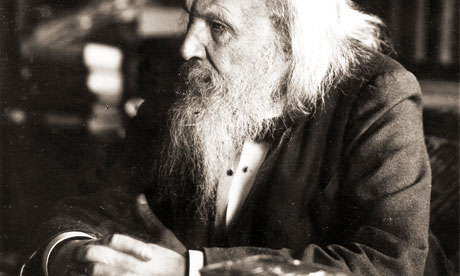
\includegraphics[width=.8\textwidth]{./pictures/mendeleev.jpg}
\caption{Photo of Dmitri Mendeleev (1834-1907). Found on The Guardian's \href{http://www.guardian.co.uk/science/blog/2011/dec/07/dmitri-mendeleev-business-card}{Notes \& Theories blog}. Public domain.}
\end{center}
\end{figure}


\subsubsection{Learning patterns}

One way to think about fun learning is that it's fun to learn new
patterns. Jürgen Schmidhuber wrote: ``A separate reinforcement learner
maximizes expected fun by finding or creating data that is better
compressible in some yet unknown but learnable way, such as jokes,
songs, paintings, or scientific observations obeying novel, unpublished
laws'' {[}4{]}. So the skateboarder enjoyed coming across new patterns
(novel tricks) that he was \emph{able} to learn; tricks that challenged
his current skill level.

\subsection{Learner, know thyself: A self-evaluation technique}

When joining the Peeragogy project, I did a brief self-evaluation about
what makes me turn on to learning:

\begin{itemize}
\item
  \emph{Context.} I resist being groomed for some unforseeable future
  rather than for a purpose.
\item
  \emph{Timing and sequence.}I find learning fun when I'm studying
  something as a way to procrastinate on another pressing assignment.
\item
  \emph{Social reinforcement.}Getting tips from peers on how to navigate
  a snowboard around moguls was more fun for me than my Dad showing me
  the proper way to buff the car's leather seats on chore day.
\item
  \emph{Visible reward}. In high school, it was not fun in the moment to
  sit and compose a 30-page reading journal for Frankenstein. But owing
  in part to those types of prior experiences, writing is now fun and
  it's a pleasure to learn how to write better.
\end{itemize}

\subsection{The role of metacognition in peer learning}

The profile of each individual participant, both from the perspective of
self-awareness, as well as from the perspective of maximal value of
contribution to the group endeavor, becomes a metacognitive inquiry into
each peeragogue's skills, talents, subject matter expertise,
socialization and suitability for the array of roles and positions
required to achieve a communally defined and framed goal or output.
``Metacognitive'' means that the peeragogue is practicing awareness of
how he or she is thinking and attending. The short form is
"\emph{Deliberate self-awareness of one's thinking processes}."

Since in principle there is no authority figure or leader to exercise
judgment or discretion regarding the above, it becomes a necessary
self-evaluative examination and declaration in regard to the group,
enabling participating individuals to maximize their engagement and
contribution to the undertaking.

\subsubsection{\textbf{Possible Roles}}

\begin{itemize}
\item
  Leader, Manager, Team Member, Worker
\item
  Content Creator, Author, Content Processor, Reviewer, Editor
\item
  Presentation Creator, Designer, Graphics, Applications
\item
  Planner, Project Manager, Coordinator, Attendee, Participant
\item
  Mediator, Moderator, Facilitator, Proponent, Advocate, Representative,
  Contributor
\end{itemize}

\subsubsection{\textbf{Possible Contributions}}

\begin{itemize}
\item
  Create, Originate, Research, Aggregate
\item
  Develop, Design, Integrate, Refine, Convert
\item
  Write, Edit, Layout
\end{itemize}

We find it useful to build in a brief pause at the commencement of the
project for each peeragogue to honestly self-define and declare to the
group what he thinks he can bring to the table as a function of his
knowledge, skills, capacities, and preferences. This process primes the
group for cohesion and success.

\subsection{Personal Learning Networks and Peer Learning Networks}

Personal Learning Networks are the collections of people and information
resources (and relationships with them) that people cultivate in order
to form their own learning networks --- living, growing, responsive
sources of information, support, and inspiration that support
self-learners.

\begin{quote}
\textbf{Howard Rheingold}:\emph{When I started using social media in the
classroom, I looked for and began to learn from more experienced
educators. First, I read and then tried to comment usefully on their
blog posts and tweets. When I began to understand who knew what in the
world of social media in education, I narrowed my focus to the most
knowledgeable and adventurous among them. I paid attention to the people
the savviest social media educators paid attention to. I added and
subtracted voices from my attention network, listened and followed, then
commented and opened conversations. When I found something I thought
would interest the friends and strangers I was learning from, I passed
along my own learning through my blogs and Twitterstream. I asked
questions, asked for help, and eventually started providing answers and
assistance to those who seemed to know less than I. The teachers I had
been learning from had a name for what I was doing --- ``growing a
personal learning network.'' So I started looking for and learning from
people who talked about HOW to grow a ``PLN'' as the enthusiasts called
them.}
\end{quote}

\subsubsection{\textbf{Strong and weak ties}}

Your PLN will have people and sites that you check on often -- your main
sources of information and learning -- your `strong ties'. Your `weak
ties' are those people and sites that you don't allow a lot of bandwidth
or time. But they may become strong over time, as your network grows or
your interests expand. This is a two-way street -- it is very important
that you are sharing what you learn and discover with those in your
network and not just taking, if you want to see your network expand.

\begin{center}
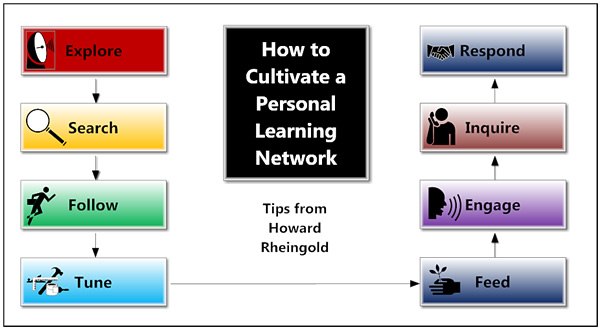
\includegraphics[width=.7\textwidth]{./pictures/Personal-Learning-Network-900px-v2.jpeg}
\end{center}

\subsubsection{Peer Learning Networks}

Later in the handbook we'll talk more about how to develop and share
``\href{http://peeragogy.org/patterns-usecases/patterns-and-heuristics/roadmap/}{peeragogical
profiles}'' -- in other words how to advertise what you want to learn,
and what you'd be interested in helping teach others. A network of
people who share their profiles and work together to
learn/teach/heal/communicate/etc. is a ``Peer Learning Network''. You'll
also find more information about building a PLN in our article on
\href{http://peeragogy.org/k-12-peeragogy/}{Peeragogy for K-12
Educators} (the article is also useful even if you're not formally
employed a teacher).

\subsection{Personal Learning Plans and Peer Learning Plans}

A PLP is designed to develop a learner's learning and teaching
capabilities. Learners learn how to develop, implement, review, and
adjust personal learning goals. The PLP supports learners in developing
knowledge and skills that will enable them to:

\begin{enumerate}
\item
  Identify appropriate future options;
\item
  Review their strengths and areas for development;
\item
  Identify goals and plans for improvement;
\item
  Monitor their actions and review and adjust plans as needed to achieve
  their goals.
\end{enumerate}

\subsubsection{\textbf{Steps in making the PLP}}

\begin{enumerate}
\item
  \emph{Learning needs:}What do you most need to learn about in the time
  ahead?
\item
  \emph{Learning activities:} What are the best ways you learn, what
  learning activities will meet your learning needs, what help will you
  need and how long will it take?
\item
  \emph{Evidence of learning:}What will you put into your personal
  portfolio to demonstrate your learning progress and achievements?
\end{enumerate}

\subsubsection{Peer Learning Plans}

On the same page where we talk about ``peeragogical profiles'', we also
talk about how to build a
"\href{http://peeragogy.org/patterns-usecases/patterns-and-heuristics/roadmap/}{shared
roadmap}'' for your peer learning project. Indeed, the idea of a
``roadmap'' is really a central pattern that comes up in this book again
and again.

\subsection{From training to learning}

\begin{figure}
\begin{center}
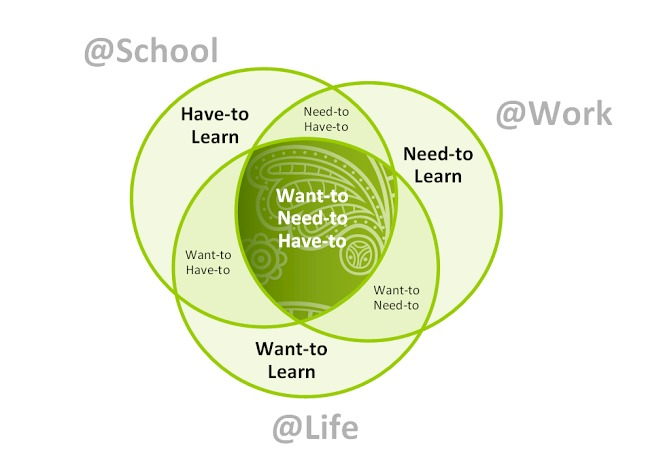
\includegraphics[width=.8\textwidth]{./pictures/learn.jpg}
\caption{``I think because of the tremendous changes we see in education and at
work, the sets (attitudes) are beginning to overlap more and more,''
said Joachim Stroh of the Google+ community, Visual Metaphors. (Used with permission)}
\end{center}
\end{figure}

The idea we develop here relates back to the question ``what makes
learning fun for me.'' In short, if it's not something that you choose,
it's not as likely to stick. However, dozen years ago, the words
\emph{training} and \emph{learning} were interchangeable, but today
\emph{learning} is revered and \emph{training} is in the dog house.
What's the difference? Training is something that's pushed on you;
someone else is in charge. Learning is something you choose to do,
whether you're being trained or not. You're in charge.

And think of all the people we learn from who aren't necessarily
trainers! Parents, grandparents, aunts, uncles, brothers, sisters,
playmates, cousins, Little Leaguers, Scouts, school chums, roommates,
teammates, classmates, study groups, coaches, bosses, mentors,
colleagues, gossips, co-workers, neighbors, and our kids\ldots{}

\emph{This has ramifications for the way people manage}. To extract
optimal performance from workers, managers must inspire them rather than
command them. Antoine de Saint-Exupéry put it nicely: ``If you want to
build a boat, do not instruct the men to saw wood, stitch the sails,
prepare the tools and organize the work, but make them long for setting
sail and travel to distant lands.'' Knowledge workers of the future will
have instant, ubiquitous access to the Net. The measure of their
learning is an open-book exam. ``What do you know?'' is replaced with
``What can you do?''.

\begin{quote}
\textbf{Jay Cross}: If I were an instructional designer in a moribund
training department, I'd polish up my resume and head over to marketing.
Co-learning can differentiate services, increase product usage,
strengthen customer relationships, and reduce the cost of hand-holding.
It's cheaper and more useful than advertising. But instead of just
making a copy of today's boring educational practices, build something
based on interaction and camaraderie, perhaps with some healthy
competition thrown in. Again, the emphasis should always be on learning
in order to do something!
\end{quote}

\subsection{Play and learning}

Once more we're back to the question, ``What makes learning fun?'' There
are deep links between play and learning. Consider, for instance, the
way we learn the rules of a game through playing it. The first times we
play a card game, or a physical sport, or a computer simulation we test
out rule boundaries as well as our understanding. Actors and
role-players learn their roles through the dynamic process of
performance. The resulting learning isn't absorbed all at once, but
accretes over time through an emergent process, one unfolding further
through iterations. In other words, the more we play a game, the more we
learn it.

In addition to the rules of play, we learn about the subject which play
represents, be it a strategy game (chess, for example) or simulation of
economic conflict. Good games echo good teaching practice, too, in that
they structure a single player's experience to fit their regime of
competence (cf. Vygotsky's zone of proximal learning, a la Gee {[}5{]}).
That is to say a game challenges players at a level suited to their
skill and knowledge: comfortable enough that play is possible, but so
challenging as to avoid boredom, eliciting player growth. Role-playing
in theater lets performers explore and test out concepts; see Boal
{[}6{]}. Further, adopting a playful attitude helps individuals meet new
challenges with curiousity, along with a readiness to mobilize ideas and
practical knowledge. Indeed, the energy activated by play can take a
person beyond an event's formal limitations, as players can assume that
play can go on and on {[}7{]}.

\begin{quote}
\textbf{Douglas Thomas and John Seely Brown}: ``All systems of play are,
at base, learning systems.'' {[}8{]}
\end{quote}

Games have always had a major social component, and learning plays a key
role in that interpersonal function. Using games to build group cohesion
is an old practice, actually a triusm in team sports.

It is important to locate our peeragogical moment in a world where
gaming is undergoing a renaissance. Not only has digital gaming become a
large industry, but gaming has begun to infiltrate non-gaming aspects of
the world, sometimes referred to as ``gamification.'' Putting all three
of these levels together, we see that we can possibly improve
co-learning by adopting a playful mindset. Such a playful attitude can
then mobilize any or all of the above advantages. For example,

\begin{itemize}
\item
  Two friends are learning the Russian language together. They invent a
  vocabulary game: one identifies an object in the world, and the other
  must name it in Russian. They take turns, each challenging the other,
  building up their common knowledge.
\item
  A middle-aged man decides to take up hiking. The prospect is somewhat
  daunting, since he's a very proud person and is easily stymied by
  learning something from scratch. So he adopts a ``trail name'', a
  playful pseudonym. This new identity lets him set-aside his
  self-importance and risk making mistakes. Gradually he grows
  comfortable with what his new persona learns.
\item
  We can also consider the \textbf{design} field as a useful kind of
  playful peeragogy. The person \emph{playing the role} of the designer
  can select the contextual frame within which the design is performed.
  This frame can be seen as the \emph{rules} governing the design, the
  artifact and the process. These rules, as with some games, may change
  over time. Therefore the possibility to adapt, to tailor one's
  activities to changing context is important when designing playful
  learning activities. (And we'll look at some ways to design peer
  learning experiences next!)
\end{itemize}

\subsection{From Peer Learning to ``Peeragogy''}

The idea that we needed a new theory (which we called \emph{paragogy})
arose out of the challenges we faced doing peer learning. Specifically,
we were particularly interested in the conditions that were required for
volunteer contributors to drive an learning-focused organization's
agenda, and improve things for participating learners and teachers. How
could the organization itself ``learn'' and grow, while participants
were also learning and becoming better contributors?

As this idea took form, we reflected more on how learning and
organizations work. Just like it would be rare for a business to be
successful if it does not take into account the needs and interests of
its clients, it is unlikely for a learning project to be successful if
the act of learning is not somehow relevant for the people doing it.

So, paragogy became \emph{a set of proposed principles} for
understanding learning (and working) together. In particular, we focused
on the way in which co-learners shape their learning context together.
Paragogy is not a recipe: its ideas can grow and change to suit the
needs of the moment; as it has matured, it has become more of an
``approach'' than it is a set of set-in-stone principles. It's also riff
on the word ``andragogy'', which comes from Malcolm Knowles. He wrote:

\begin{quote}
\emph{{[}A{]}ndragogy is simply another model of assumptions about adult
learners to be used alongside the pedagogical model of assumptions,
thereby providing two alternative models for testing out the assumptions
as to their `fit' with particular situations. Furthermore, the models
are probably most useful when seen not as dichotomous but rather as two
ends of a spectrum , with a realistic assumption (about learners) in a
given situation falling in between the two ends} {[}9{]} (p. 43).
\end{quote}

We also tried, at least at first, to be similarly non-oppositional with
respect to andragogy:

\begin{quote}
\emph{{[}T{]}he most important initial condition in andragogy seems to
be that an adult educator or facilitator is part of the picture. In a
peer-based setting, that may not be the case: we can easily find
examples of learning environments where there is no ``teacher'' in the
``classroom''; where, for example, the task of facilitation is shared
among all participants or even encoded in the learning materials or
supportive technologies. Not that one way is more desirable than
another: we simply mean to highlight the fact that the most basic
features of a given learning environment will influence everything
else.} {[}10{]}
\end{quote}

``Paragogy'' is intended to be a broad, inclusive, and purposefully
ambiguous term. ``Peeragogy'' by contrast attempts to make the idea more
concrete and immediately understandable: peeragogy is about peers
learning together, and teaching each other. In the end, the two words
are actually synonyms. If you prefer to go merrily into theory-building
mode, feel free to spell it ``paragogy''. If you want to be a bit more
down to earth, use ``peeragogy.''

\subsubsection{Different ways to analyze the learning process}

Since we are interested in how students (and others) can collaborate in
learning, bringing to their own particular experiences, strengths, and
weaknesses to bear, we ask: ``How can each participant contribute to a
group in their own way? Which kind of activities can we design to foster
``multi-modal'' collaborative learning, and how do we assess the
outcomes?'' One approach is to look at the ``multiple different social
roles'' which people take on in educational contexts:

\begin{quote}
\emph{{[}W{]}e use {[}Ken{]} Wilber's terms to describe a given social
role in terms of its constituent actions. So for example, the role of
``being a student'' might be described as follows: ``\textbf{I}}\emph{go
to class, \textbf{we}}\emph{do a class project, the objects of concern
(``\textbf{Its}}\emph{'') are things I can add to my portfolio or
work-record; and fundamentally, \textbf{it}}\emph{is all about gaining a
skill.'' This simple background story gives us a notion of role,
persona, or identity: a role that is defined by its constituent actions,
relative a given social context. And here, context is conceived of,
after Nishida, as a ``shared context in motion.''} {[}11{]}
\end{quote}

After doing some personal reflection on the roles you want to take on
and the contributions you want to make (as we discussed above), you may
also want to work together with your learning group to analyze the
learning process in more detail. There are many different phases,
stages, and dimensions that you can use to help structure and understand
the learning experience: we list some of these below.

\begin{itemize}
\item
  \emph{Guidance \& Support}, \emph{Communication \& Collaboration},
  \emph{Reflection \& Demonstration}, \emph{Content \& Activities} (from
  Gráinne Conole)
\item
  \emph{Forming}, \emph{Norming}, \emph{Storming}, \emph{Performing}
  from Bruce Tuckman.
\item
  The ``five-stage e-moderating model'' from GIlly Salmon
\item
  \emph{Assimilative, Information Processing, Communicative, Productive,
  Experiential, Adaptive}(from Oliver and Conole)
\item
  Multiple intelligences (after Howard Gardner).
\item
  The associated ``mental state''(after Csíkszentmihályi; see
  picture)\emph{}
\item
  Considered in terms of ``Learning Power'' (Deakin-Crick, Broadfoot,
  and Claxton).
\end{itemize}

\begin{figure}
\begin{center}
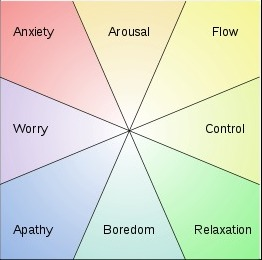
\includegraphics[width=.5\textwidth]{./pictures/challenge.jpg} 
\end{center}
\caption{
\href{http://commons.wikimedia.org/wiki/File\%3AChallenge\_vs\_skill.svg}{Challenge vs. Skill}. By w:User:Oliverbeatson (w:File:Challenge vs skill.jpg)
{[}Public domain{]}}
\end{figure}

\subsection{Further reading}

\subsubsection{A word list for your inner edu-geek}

\begin{itemize}
\item
  Constructivism
\item
  Social constructivism
\item
  Radical constructivism
\item
  Enactivism
\item
  Constructionism
\item
  Connectivism
\end{itemize}

\subsubsection{On fun and boredom}

\begin{itemize}
\item
  \emph{The Contribution of Judo to Education} by Kano Jigoro
\item
  \emph{Pale King}, unfinished novel by David Foster Wallace,
\end{itemize}

\subsubsection{On Paragogy}

\begin{itemize}
\item
  Joe Corneli's
  ``\href{http://en.wikiversity.org/wiki/User:Arided/ImplementingParagogy}{Implementing
  Paragogy}'' lesson plan, on Wikiversity
\item
  Joe Corneli and Charlie Danoff's ``Paragogy Papers'', on
  \href{paragogy.net}{paragogy.net}
\end{itemize}

\subsubsection{on Learning vs Training}

\begin{itemize}
\item
  Hart, Jane.
  \href{http://www.c4lpt.co.uk/blog/2012/04/20/is-it-time-for-a-byol-bring-your-own-learning-strategy-in-your-organization-byol/}{Is
  it time for a BYOL (Bring Your Own Learning) strategy for your
  organization}?
\end{itemize}

\subsubsection{on PLNs}

\begin{itemize}
\item
  \href{http://dmlcentral.net/blog/howard-rheingold/shelly-terrell-global-netweaver-curator-pln-builder}{Shelly
  Terrell: Global Netweaver, Curator, PLN Builder}, blog post, with
  video
\item
  Will Richardson and Rob Mancabelli,
  \href{http://weblogg-ed.com/2011/personal-learning-networks-an-excerpt/}{Personal
  Learning Networks: Using the Power of Connection to Transform
  Education}
\item
  \href{http://delicious.com/hrheingold/pln}{Howard Rheingold's PLN
  links on Delicious}
\end{itemize}

\subsubsection{Exercises to help cultivate a playful attitude}

\begin{itemize}
\item
  Use the \href{http://www.rtqe.net/ObliqueStrategies/}{Oblique
  Strategies} card deck (Brian Eno and Peter Schmidt, 1st edition 1975,
  now available in its fifth edition) to spur playful creativity. Each
  card advises players to change their creative process, often in
  surprising directions.
\item
  Take turns making and sharing videos. This online collaborative
  continuous video storytelling involves a group of people creating
  short videos, uploading them to YouTube, then making playlists of
  results. Similar to \href{http://clipkino.info/}{Clip Kino}, only
  online.
\item
  Engage in theater play using Google+ Hangout. e.g. coming together
  with a group of people online and performing theatrical performances
  on a shared topic that are recorded.
\end{itemize}

\subsection{References}

\begin{enumerate}
\item
  Dewey, J. (2004). \emph{Democracy and education}. Dover Publications.
\item
  Vygotsky, L. S. (1986). \emph{Thought and language}. MIT press.
\item
  Siemens, G. (2005). Connectivism: A learning theory for the digital
  age. \emph{International Journal of Instructional Technology and
  Distance Learning}, 2(1), 3-10.
\item
  Schmidhuber, J. (2010). Formal theory of creativity, fun, and
  intrinsic motivation. \emph{Autonomous Mental Development (IEEE)},
  2(3), 230-247.
\item
  Gee, J. P. (1992). \emph{The social mind: Language, ideology, and
  social practice}. Series in language and ideology. New York: Bergin \&
  Garvey.
\item
  Boal, A. (1979). \emph{Theatre of the oppressed}. 3rd ed. London:
  Pluto Press.
\item
  Bereiter, C. and Scadamalia, M. (1993). \emph{Surpassing ourselves,
  an~inquiry into the nature and implications of expertise}. Peru,
  Illinois:~Open Court.
\item
  Douglas Thomas and John Seely Brown (2011), \emph{A New Culture of
  Learning: Cultivating the Imagination for a World of Constant Change}.
  CreateSpace.
\item
  Knowles, M. S. (1980). The modern practice of adult education: From
  pedagogy to andragogy. Chicago: Follett.
\item
  Corneli, J. and Danoff, C.J. (2011), Paragogy: Synergizing individual
  and organizational learning. (Published
  \href{\%20http://en.wikiversity.org/wiki/User:Arided/ParagogyPaper}{on
  Wikiversity}.)
\item
  Corneli, J., \& Mikroyannidis, A. (2012). Crowdsourcing education on
  the Web: a role-based analysis of online learning communities, in
  Alexandra Okada, Teresa Conolly, and Peter Scott (eds.),
  \emph{Collaborative Learning 2.0: Open Educational Resources}, IGI
  Global.
\end{enumerate}

~
